% Introduction

\chapter{Introduction}

Specialized hardware for running deep learning algorithms seems to be a natural step in the evolution of
Artificial Intelligence.  Google, for example, developed its own \gls{asic} named Tensor Processing Unit (TPU)
to accelerate tensor computations. The formidable cost of such endeavors limits \gls{asic} development to
the big players in the industry. For tech startups and hobbyists, the \gls{fpga} comes to rescue by filling
the gap between high-cost customized ICs and the need to make specialized hardware for certain
applications. The programmable logic blocks contained in the FPGA can be reconfigured, making it ideal for
situations where "in the field" functionality update is required. It is also a valuable tool for fast
prototyping and verification of ASIC design with low cost.

Generative models are a class of algorithms which, instead of processing real world input, create fresh and
new output that resembles the real world data. They can be thought as the opposite of discriminative models,
which analyze input and compute output. In other words, generative models enable the machine to paint new
paintings, compose new music, or write new poetries. Many types of generative models exist, including deep
belief networks, variational autoencoder, Boltzmann machine, etc. They are widely used in machine learning
to model data.

\gls{gans} are a class of neural networks in which two different networks are trained to compete against
each other in order to learn about the probability distribution of a particular dataset. The training
process pits the two players in a minimax game so that the performance of both networks can improve over
time. Introduced in 2014 by Ian Goodfellow \textit{et al}. \cite{goodfellow:gan}, it soon gained popularity
in the machine learning community, kindled a wave of research on improving the training property and
quality of generation of GANs.

The marriage of FPGA and GANs seems to be an interesting topic in its own right. This project explores such
possibilities by implementing a pre-trained generator model of Deep Convolutional GANs (DCGAN) proposed by
Alec Radford \textit{et al}. \cite{radford:conv_gan} on FPGA to generate realistic pictures.
\ref{fig:bedroom} shows a group of generated images of bedrooms.

\begin{figure}[h]
  \centering
  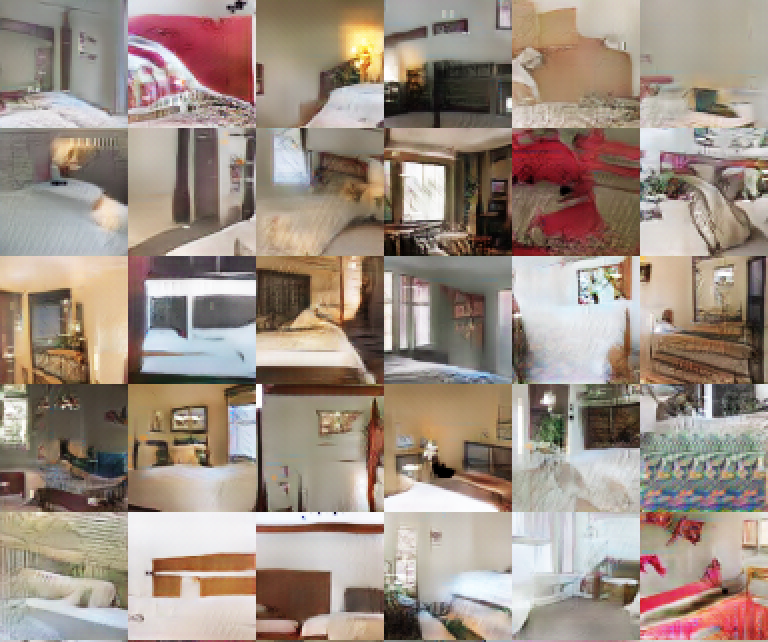
\includegraphics[scale=0.5]{bedroom}
  \caption{Images of bedrooms generated by DCGAN}
  \label{fig:bedroom}
\end{figure}

Nowadays High Level Synthesis (HLS) is a quite popular option for implementing algorithms on FPGA. HLS takes a
behavioral description written in a high-level programming language such as C and translates the description
into register-transfer level (RTL) hardware description language (HDL) such as Verilog or VHDL. This approach
is particularly favoured by software engineers who wish to quickly convert a software program into
hardware implementation. In this project however, we choose to use the low-level HDL to implement the
generator model to gain finer control of the implementation details. A näive Verilog version is presented
first, then several optimization possibilities are experimented. This paper serves as a rather detailed
documentation of the design and implementation process. The core Verilog module can be found in Appendix 1,
which is annotated with comments.

The generator is a deep \gls{cnn}. In such networks a large part of the computation is done with an
operation called the \gls{gemm}. Therefore, an efficient implementation of GEMM is crucial to the
acceleration. However, CNNs are normally implemented with floating-point numbers, which are much less
efficient to handle in hardware than fixed-point numbers. If only we could carry out the computation in
fixed-point numbers and then convert the result back to floating-point numbers! Such techniques do exist
and they are referred to as quantization, which is the key to realize high performance in hardware. Chapter 5
provides a detailed discussion of the quantization scheme used in this project.

\clearpage %force the next chapter to start on a new page. Keep that as the last line of your chapter!
